\documentclass[12pt, letterpaper, twoside]{article}
\usepackage[margin=0.9in]{geometry}

\usepackage[utf8]{inputenc}
\usepackage[portuguese]{babel}
\usepackage{mlmath}
\usepackage{amssymb}
\usepackage{xcolor}
\usepackage{minted}
\usemintedstyle{vs}
\usepackage{multicol}
\usepackage{float}
\usepackage{tabularx}
\usepackage{graphicx}
\usepackage{amsmath}
\usepackage[]{mdframed} % Caixas de texto %
\usepackage{indentfirst} % Adiciona um tab no primeiro parágrafo%
\usepackage{booktabs}
\usepackage{hyperref}
\usepackage{textcomp}
\usepackage{enumitem}
\usepackage{nicematrix}
\usepackage[portuguese, ruled, linesnumbered]{algorithm2e}
% Para diagramas com o TikZ
\usepackage{tikz}
\usetikzlibrary{positioning}
\usepackage{array}

% Para syntax highlight de código
\usepackage{listings}


\begin{document}

\title{CAUSP LOCK}
\author{Henrique S. Souza, Mateus Kosicov, Matheus Guidoni}

\maketitle

\section{Introdução}
Este relatório documenta o Sistema de Controle de Acesso CAUSP-LOCK, desde sua concepção de alto nível até sua implementação prática. Trata-se de um conjunto de sistemas de hardware e software suficientes para garantir o acesso de múltiplos usuários a um mesmo espaço físico, nesse caso, a sala de apoio à amamentação e regulação sensorial da Faculdade de Direito da USP, localizada em seu prédio histórico, no centro de São Paulo e destinada especialmente à comunidade autista e neurodivergente. O nome "CAUSP" de CAUSP-LOCK é referência ao Coletivo Autista da USP, do qual o Henrique S. Souza faz parte.

O hardware consiste primordialmente em uma fechadura eletrônica capaz de ler e interpretar QR Codes em um protocolo próprio. Ela é composta por três principais componentes: (i) um microcontrolador ESP32-CAM, (ii) uma câmera OV2640, e (iii) uma fechadura elétrica. O ESP32-CAM controla a câmera, que, por sua vez, efetua a captura das imagens dos QR Codes, e, caso o acesso seja autorizado, aciona a abertura da fechadura elétrica. Há um circuito elétrico de interface entre o ESP32-CAM e a fechadura elétrica, necessário para o acionamento do mecanismo, pois o microcontrolador é um dispositivo de baixa potência, com saída de 3.3V, enquanto que a fechadura demanda cerca de 12V e 1A por 1s.

O software é constituído por um (i) frontend comum, disponibilizado na forma de uma página web ou um aplicativo mobile, (ii) uma API de criação de QR Codes e (iii) um banco de dados relacional. O cliente deve cadastrar-se pelo frontend; após o cadastro ser validado, segundo uma política administrativa, e registrado no banco de dados ele terá o poder de solicitar ao sistema permissão para acessar o espaço físico. Se concedida, o que pode ou não ser automático a depender do administrador, a API gera um QR Code de acesso e o disponibiliza pelo frontend.

Para promover segurança do espaço físico, o CAUSP-LOCK gera QR Codes de acesso de uso único, temporário e assinados digitalmente, com algoritmo criptograficamente seguro, o que garante autenticidade, integridade e irretratabilidade dos acessos. A chave criptográfica empregada na assinatura é compartilhada entre o microcontrolador e o backend da aplicação assincronamente. Portanto, a tranca eletrônica funciona offline, sem necessidade de internet para autenticar os códigos de acesso dos QR Codes.

\section{Situação problema}
Desde 2024, a Faculdade de Direito do Largo de São Francisco (SanFran) possui uma sala de apoio à amamentação e regulação sensorial (vide \href{https://direito.usp.br/noticia/e59450c2bb90-fdusp-tera-sala-de-apoio-a-amamentacao-e-de-regulacao-sensorial}{link da matéria}), que faz parte de uma política de inclusão e pertencimento para autistas e mães. Como contam os diretores Celso Campilongo e Ana Elisa Bechara:

\begin{quote}
    "Nossa sala é equipada com uma variedade de estímulos sensoriais controlados. Estes elementos foram projetados para ajudar à pessoa neurodivergente a se autorregular, promovendo o bem-estar emocional e cognitivo durante a jornada acadêmica e laboral"
\end{quote}

Portanto, a sala promove o bem-estar da comunidade neurodivergente, especialmente a autista, além de gestantes. O projeto foi viabilizado graças à parceria estabelecida entre a faculdade e a Associação Nacional para Inclusão de Pessoas Autistas.

No entanto, a sala enfrenta problemas de subutilização e inacessibilidade. Por conta de a faculdade sofrer em grande medida problemas com furtos em todas as suas dependências e, por estar num prédio público, intencionalmente sem controle de acesso, ela é altamente vulnerável a mau uso e furtos de seus itens internos. Por isso, ela permanece trancada e, para acessá-la, o aluno deve pedir as chaves aos funcionários, nos corredores do 3º andar, em que a sala está localizada. Nesse contexto, há relatos de constrangimentos e dificuldades dos alunos autistas ao tentarem esse processo, por conta de alguns funcionários não concederem acesso às chaves sem um critério bem definido ou formalizado.

\section{Proposta}
Diante desse problema, esse trabalho propõe um sistema de controle de acesso baseado em uma tranca eletrônica de uso compartilhado e público, capaz de garantir a entrada facilitada, inclusiva e conveniente aos autistas e às mães no espaço sensorial, tal qual explicitado pelas figuras \ref{fig:general_view} e \ref{fig:complete_system}.

\begin{figure}
    \centering
    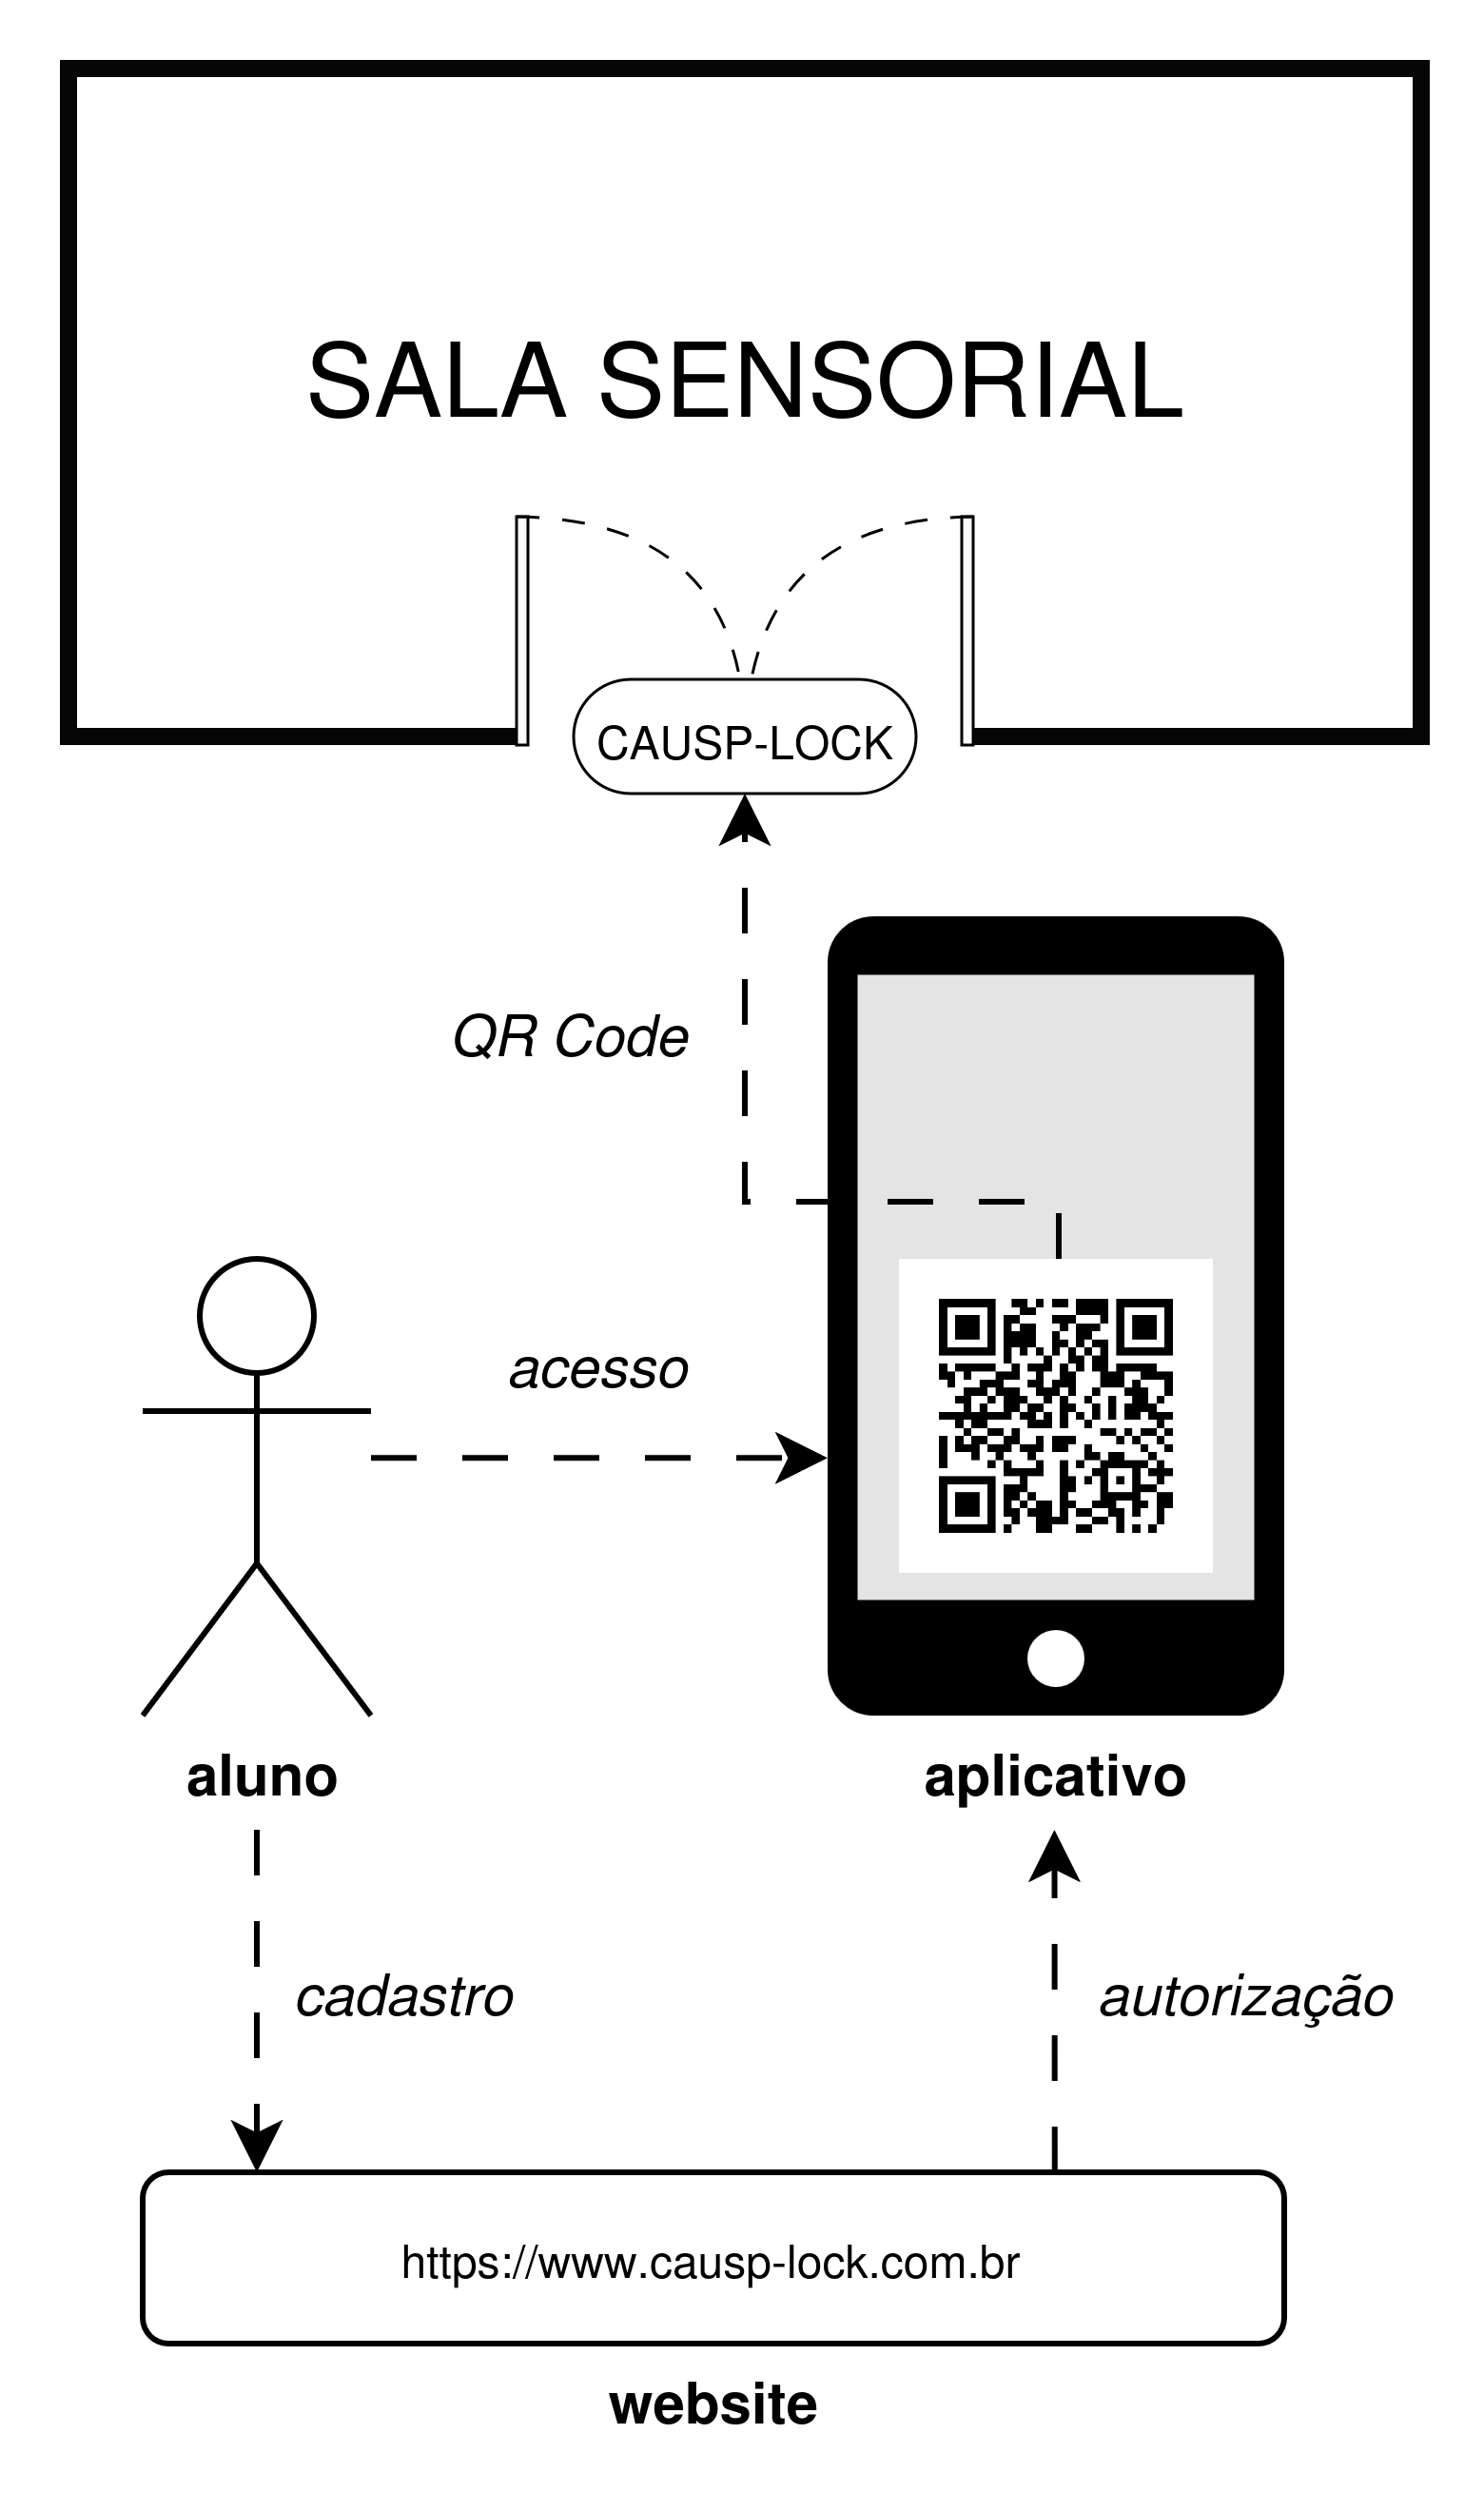
\includegraphics[width=6cm]{images/causp-lock-protocol-GENERAL_VIEW.png}
    \caption{Visão Geral do CAUSP-LOCK}
    \label{fig:general_view}
\end{figure}

A tranca apresenta um mecanismo de autenticação e autorização baseado na apresentação de QR Codes de acesso à câmera embutida no dispositivo. Os usuários terão acesso a esses QR Codes por meio de um website ou aplicativo, administrado pela SanFran de forma simplificada, com o pré-cadastro de alunos neurodivergentes e mães, a fim de facilitar o acesso. Cada QR Code é assinado com um algoritmo de criptografia simétrica, com um conjunto de chaves secretas compartilhadas apenas pelo dispositivo e pelo sistema gerador dos QR Codes. A tranca eletrônica também se responsabiliza por garantir a integridade e a autenticidade dos códigos, além de impor as limitações de uso único e expiração programada. Almeja-se, com esse sistema, facilitar o acesso à sala de amamentação e regulação sensorial, minimizando o esforço e os eventuais constrangimentos aos usuários e, ao mesmo tempo, garantir a segurança e o bom uso da sala.

\section{Arquitetura do Sistema}
O sistema abrange uma variedade de dispositivos físicos, mecânicos, elétricos e eletrônicos, e softwares, conforme ilustra a figura \ref{fig:complete_system}. Os usuários interagem com uma interface web feita em React, por meio da qual é possível, para os clientes, cadastrar-se, solicitar acesso à sala e obter QR Codes de acesso e, para os administradores, consultar os usuários cadastrados, todo o histórico de acessos da sala, conceder ou negar acesso aos clientes, controlar a concorrência, não permitindo que muitas pessoas tentem usar a sala ao mesmo tempo. O site comunica-se com uma API do python, implementada em FastAPI, para gerar os QR Codes e interagir com o banco de dados em SQL, em que se armazenam as informações dos usuários, das chaves secretas, e do histórico de uso da sala.

\begin{figure}
    \centering
    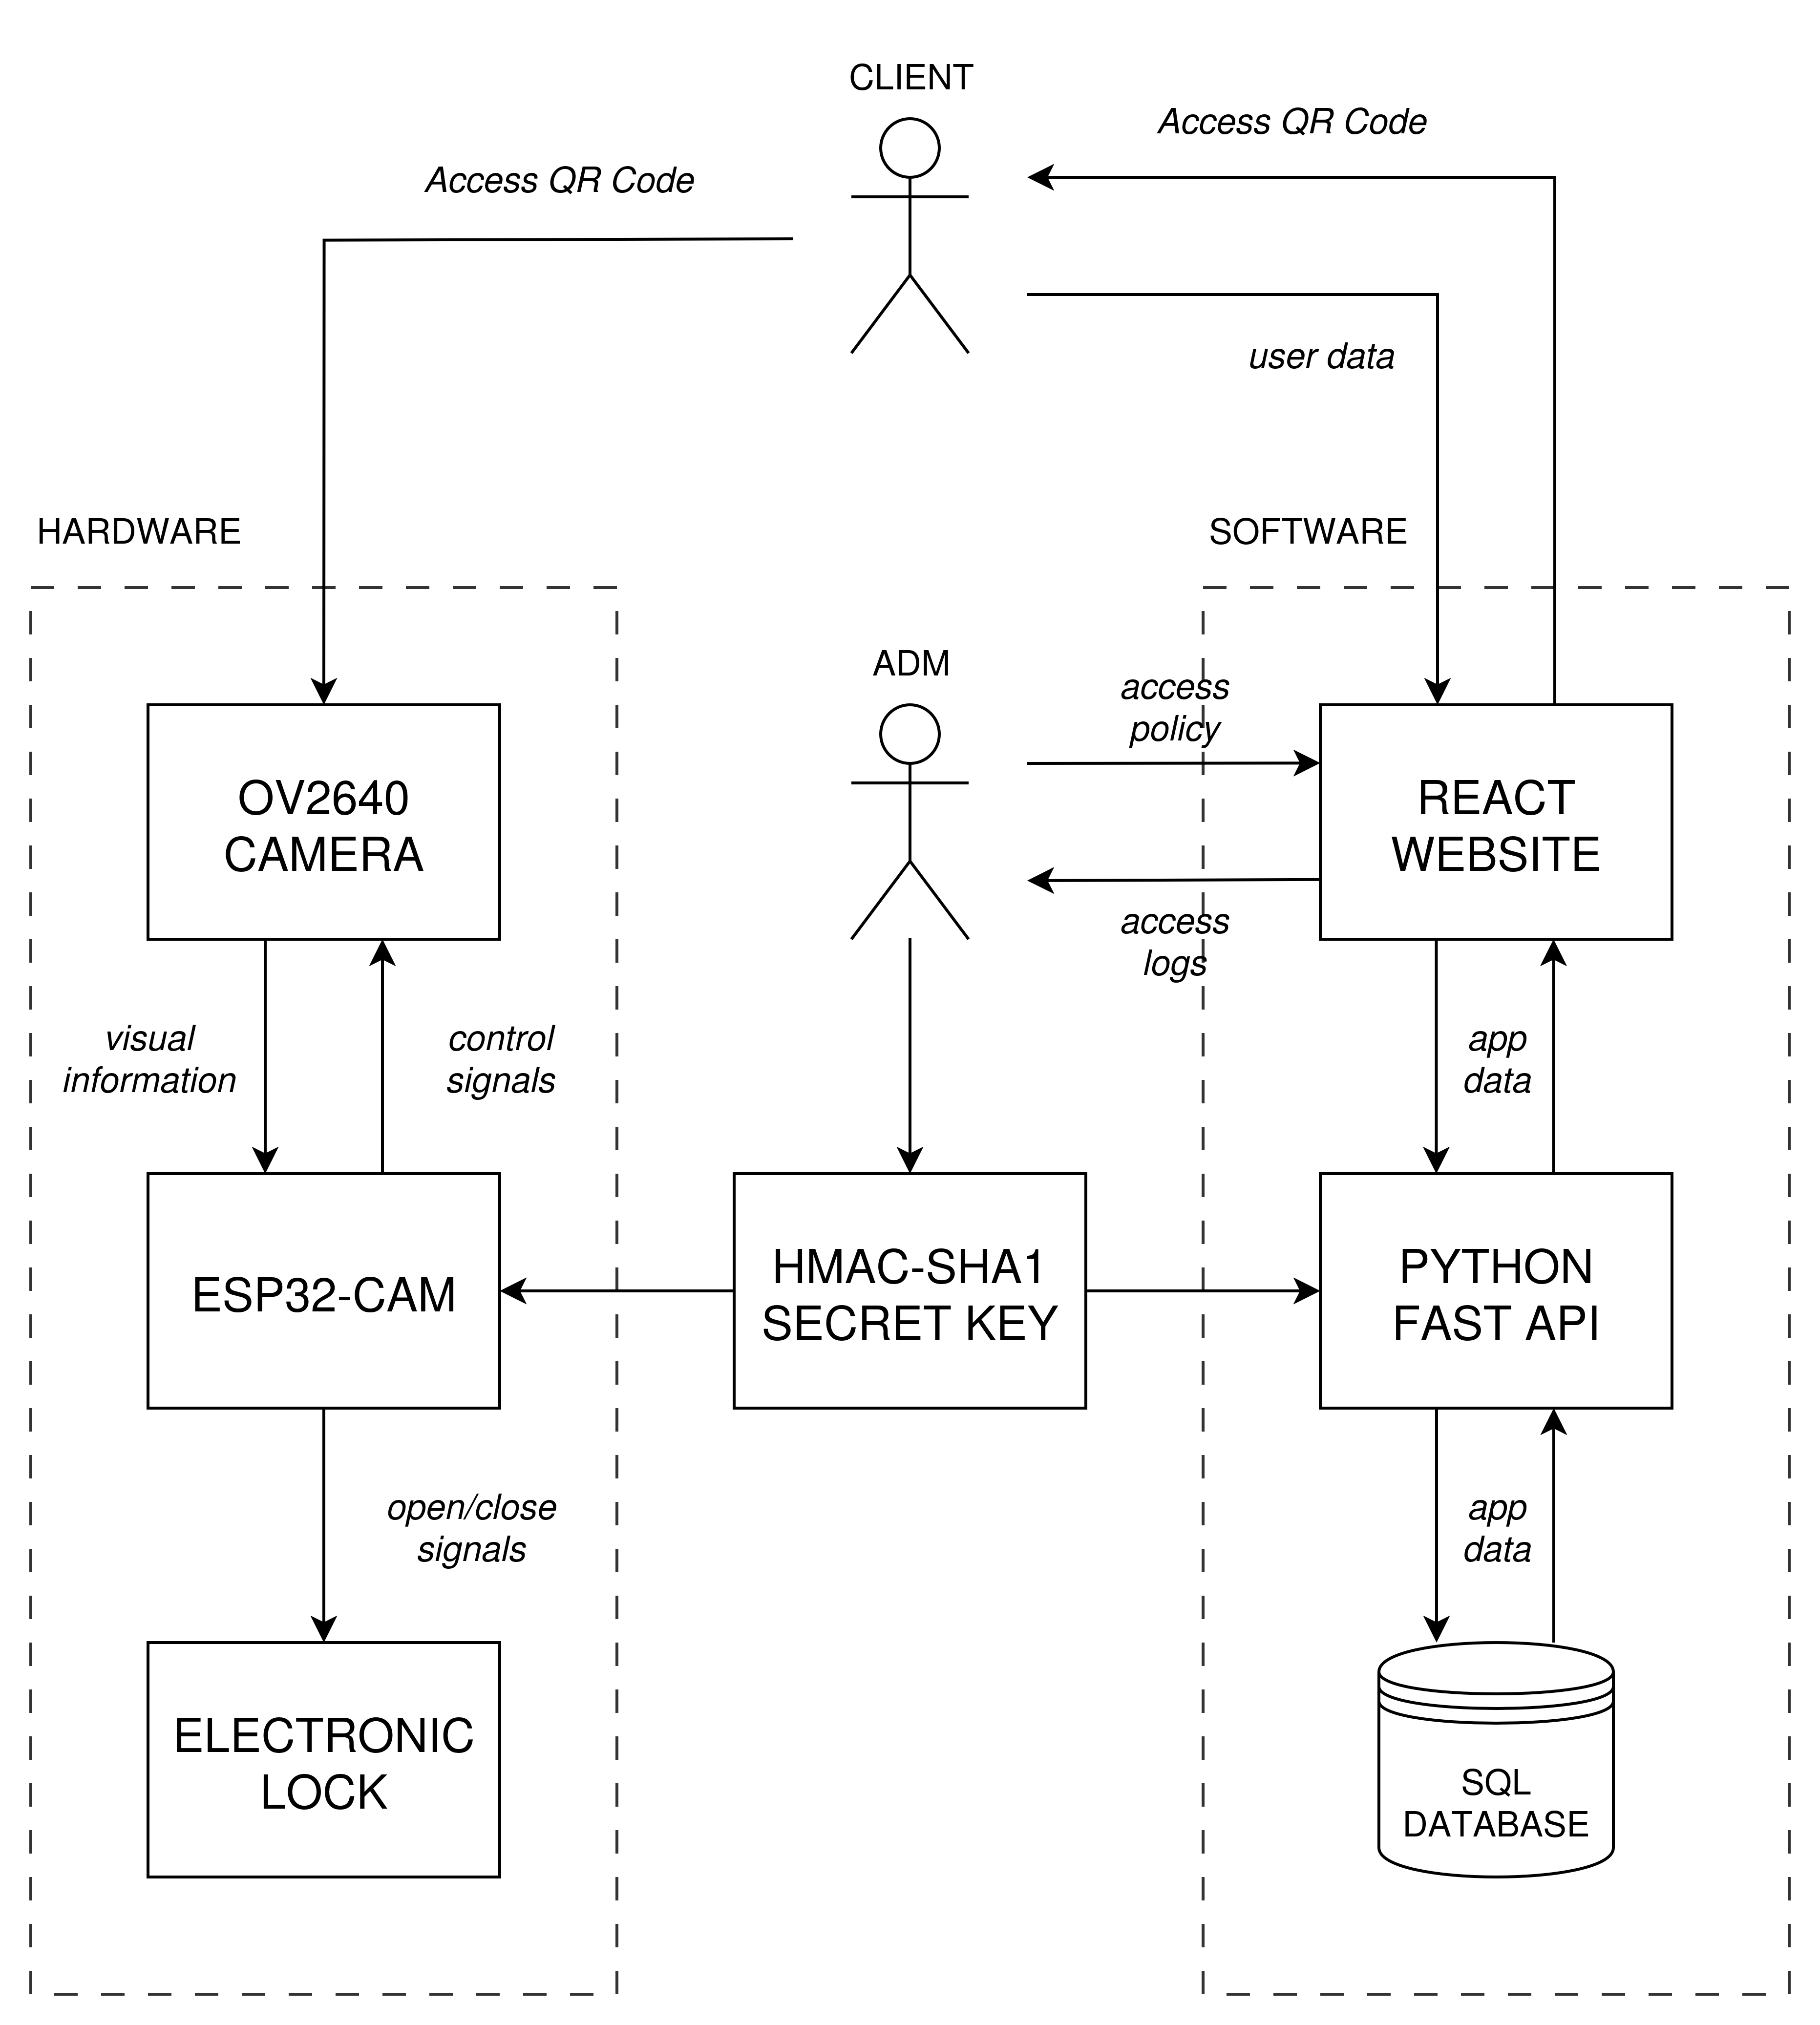
\includegraphics[width=16cm]{images/causp-lock-protocol-COMPLETE_SYSTEM.png}
    \caption{Arquitetura completa do sistema}
    \label{fig:complete_system}
\end{figure}

Ao obter os QR Codes de acesso, os clientes irão até a sala de regulação sensorial e os apresentarão à câmera OV2640, conectada ao ESP32-CAM. Então, o algoritmo fará a decodificação do QR Code em bytes, a interpretação desses bytes em dados de alto nível, a validação das assinaturas digitais HMAC-SHA1 e converterá isso em ações, por exemplo, abertura da fechadura elétrica, registro de entrada ou saída do cliente no armazenamento interno, etc.

Um aspecto importante da solução é que não há comunicação direta entre os dispositivos físicos e os serviços web. Essa escolha justifica-se por simplificar o funcionamento do acesso à sala, que, dessa forma, poderá ocorrer sem que o ESP32-CAM tenha acesso à internet. No entanto, isso também gera o trade-off de demandar dos administradores configurar os sistema web e o físico com as mesmas chaves de autenticação HMAC-SHA1.

\section{Protocolo de Comunicação via QR Codes}
A geração de QR Codes envolve codificar dados em um payload, que será então convertido numa imagem. Há diversas formas de se fazer isso, mas é necessário garantir uma codificação consistente, para que a leitura do QR Code permita decodificar o payload em seus dados originais. Para tal fim, desenvolveu-se um protocolo de comunicação via QR Codes, que define uma codificação padrão para os payloads, o que permite uma decodificação simples.

\begin{figure}[H]
    \centering
    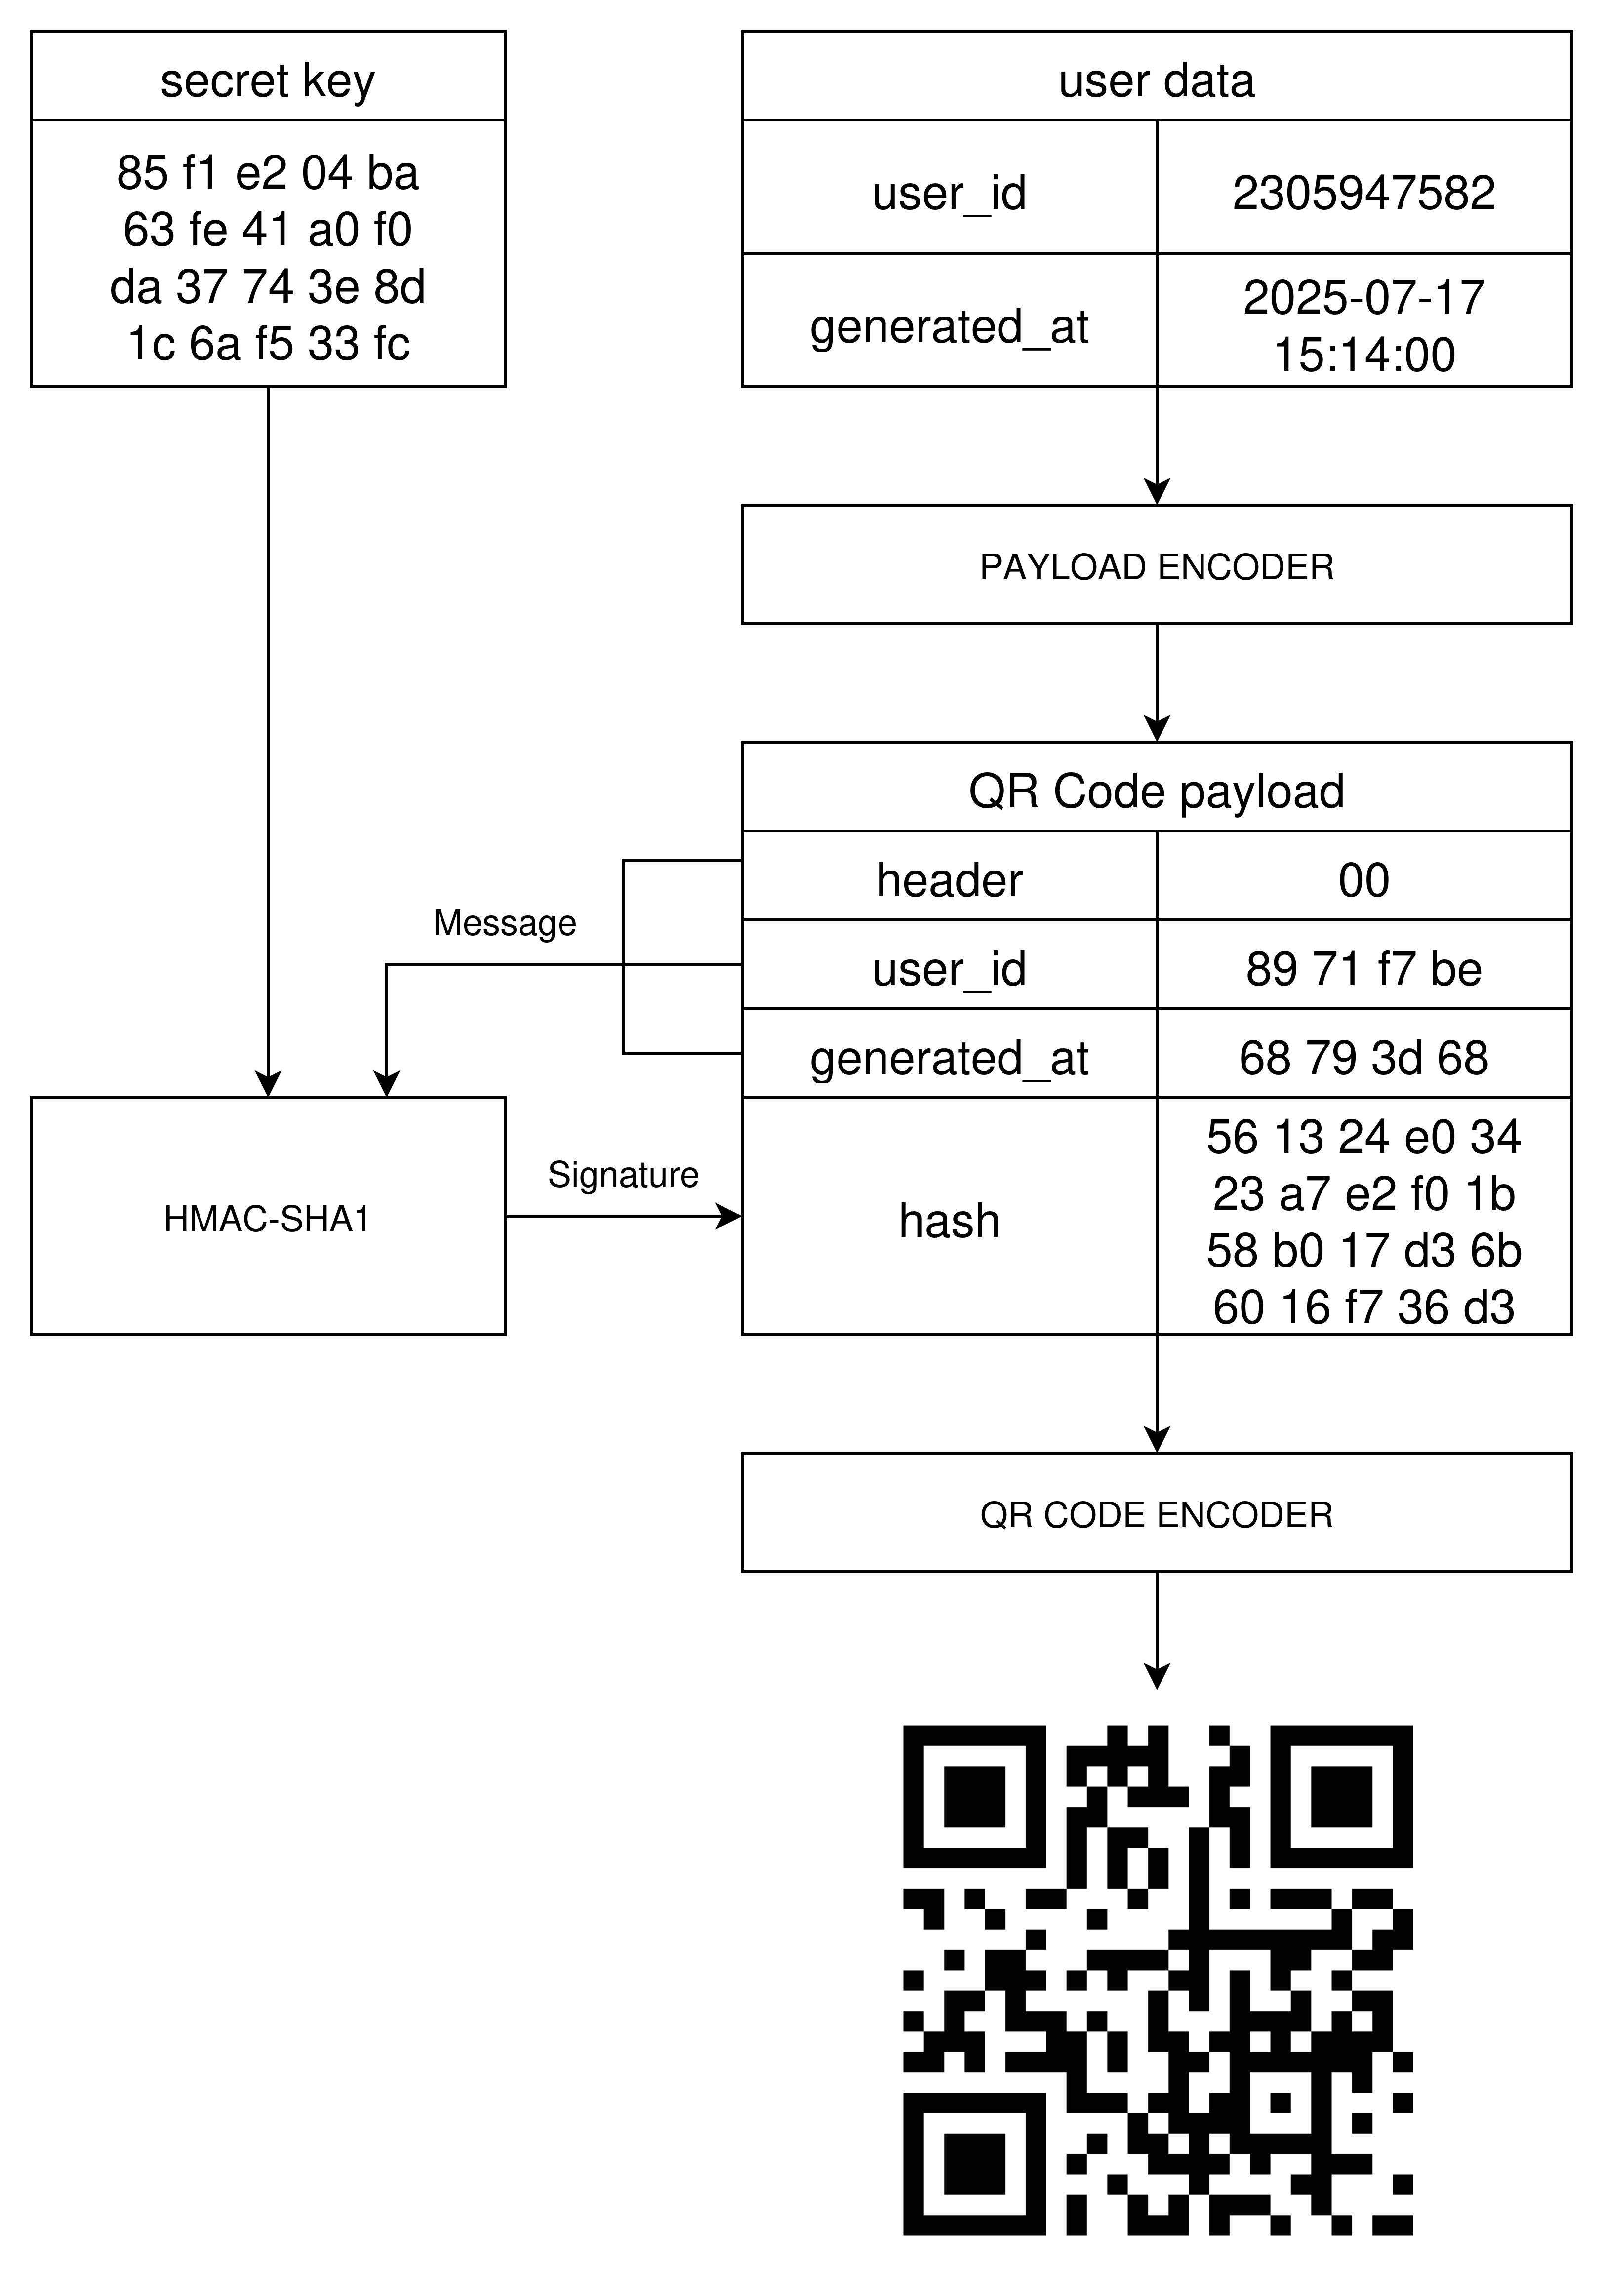
\includegraphics[width=12cm]{images/causp-lock-protocol-DATA_ENCODING.png}
    \caption{Codificação dos QR Codes}
    \label{fig:data_encoding}
\end{figure}

Conforme apresentado na figura \ref{fig:payload_encoding}, a codificação do payload, inspirada pelo datagrama do TCP, apresenta três sessões: (i) HEADER, (ii) BODY e (iii) HASH. O HEADER é o cabeçalho da mensagem e identifica seu tipo (acesso, sincronização, configuração ou depuração); seu tamanho é fixo em 1 byte. O BODY é o campo em que se colocam os dados; por exemplo, o id do usuário e o tempo em que o QR Code foi gerado, no caso de uma mensagem de acesso; seu tamanho é variado, podendo ocupar de 4 a 20 bytes. O HASH é a assinatura digital HMAC-SHA1 da mensagem e possui tamanho fixo de 20 bytes. O QR Code como um todo apresenta de 5 a 41 bytes, o total.

\begin{figure}[H]
    \centering
    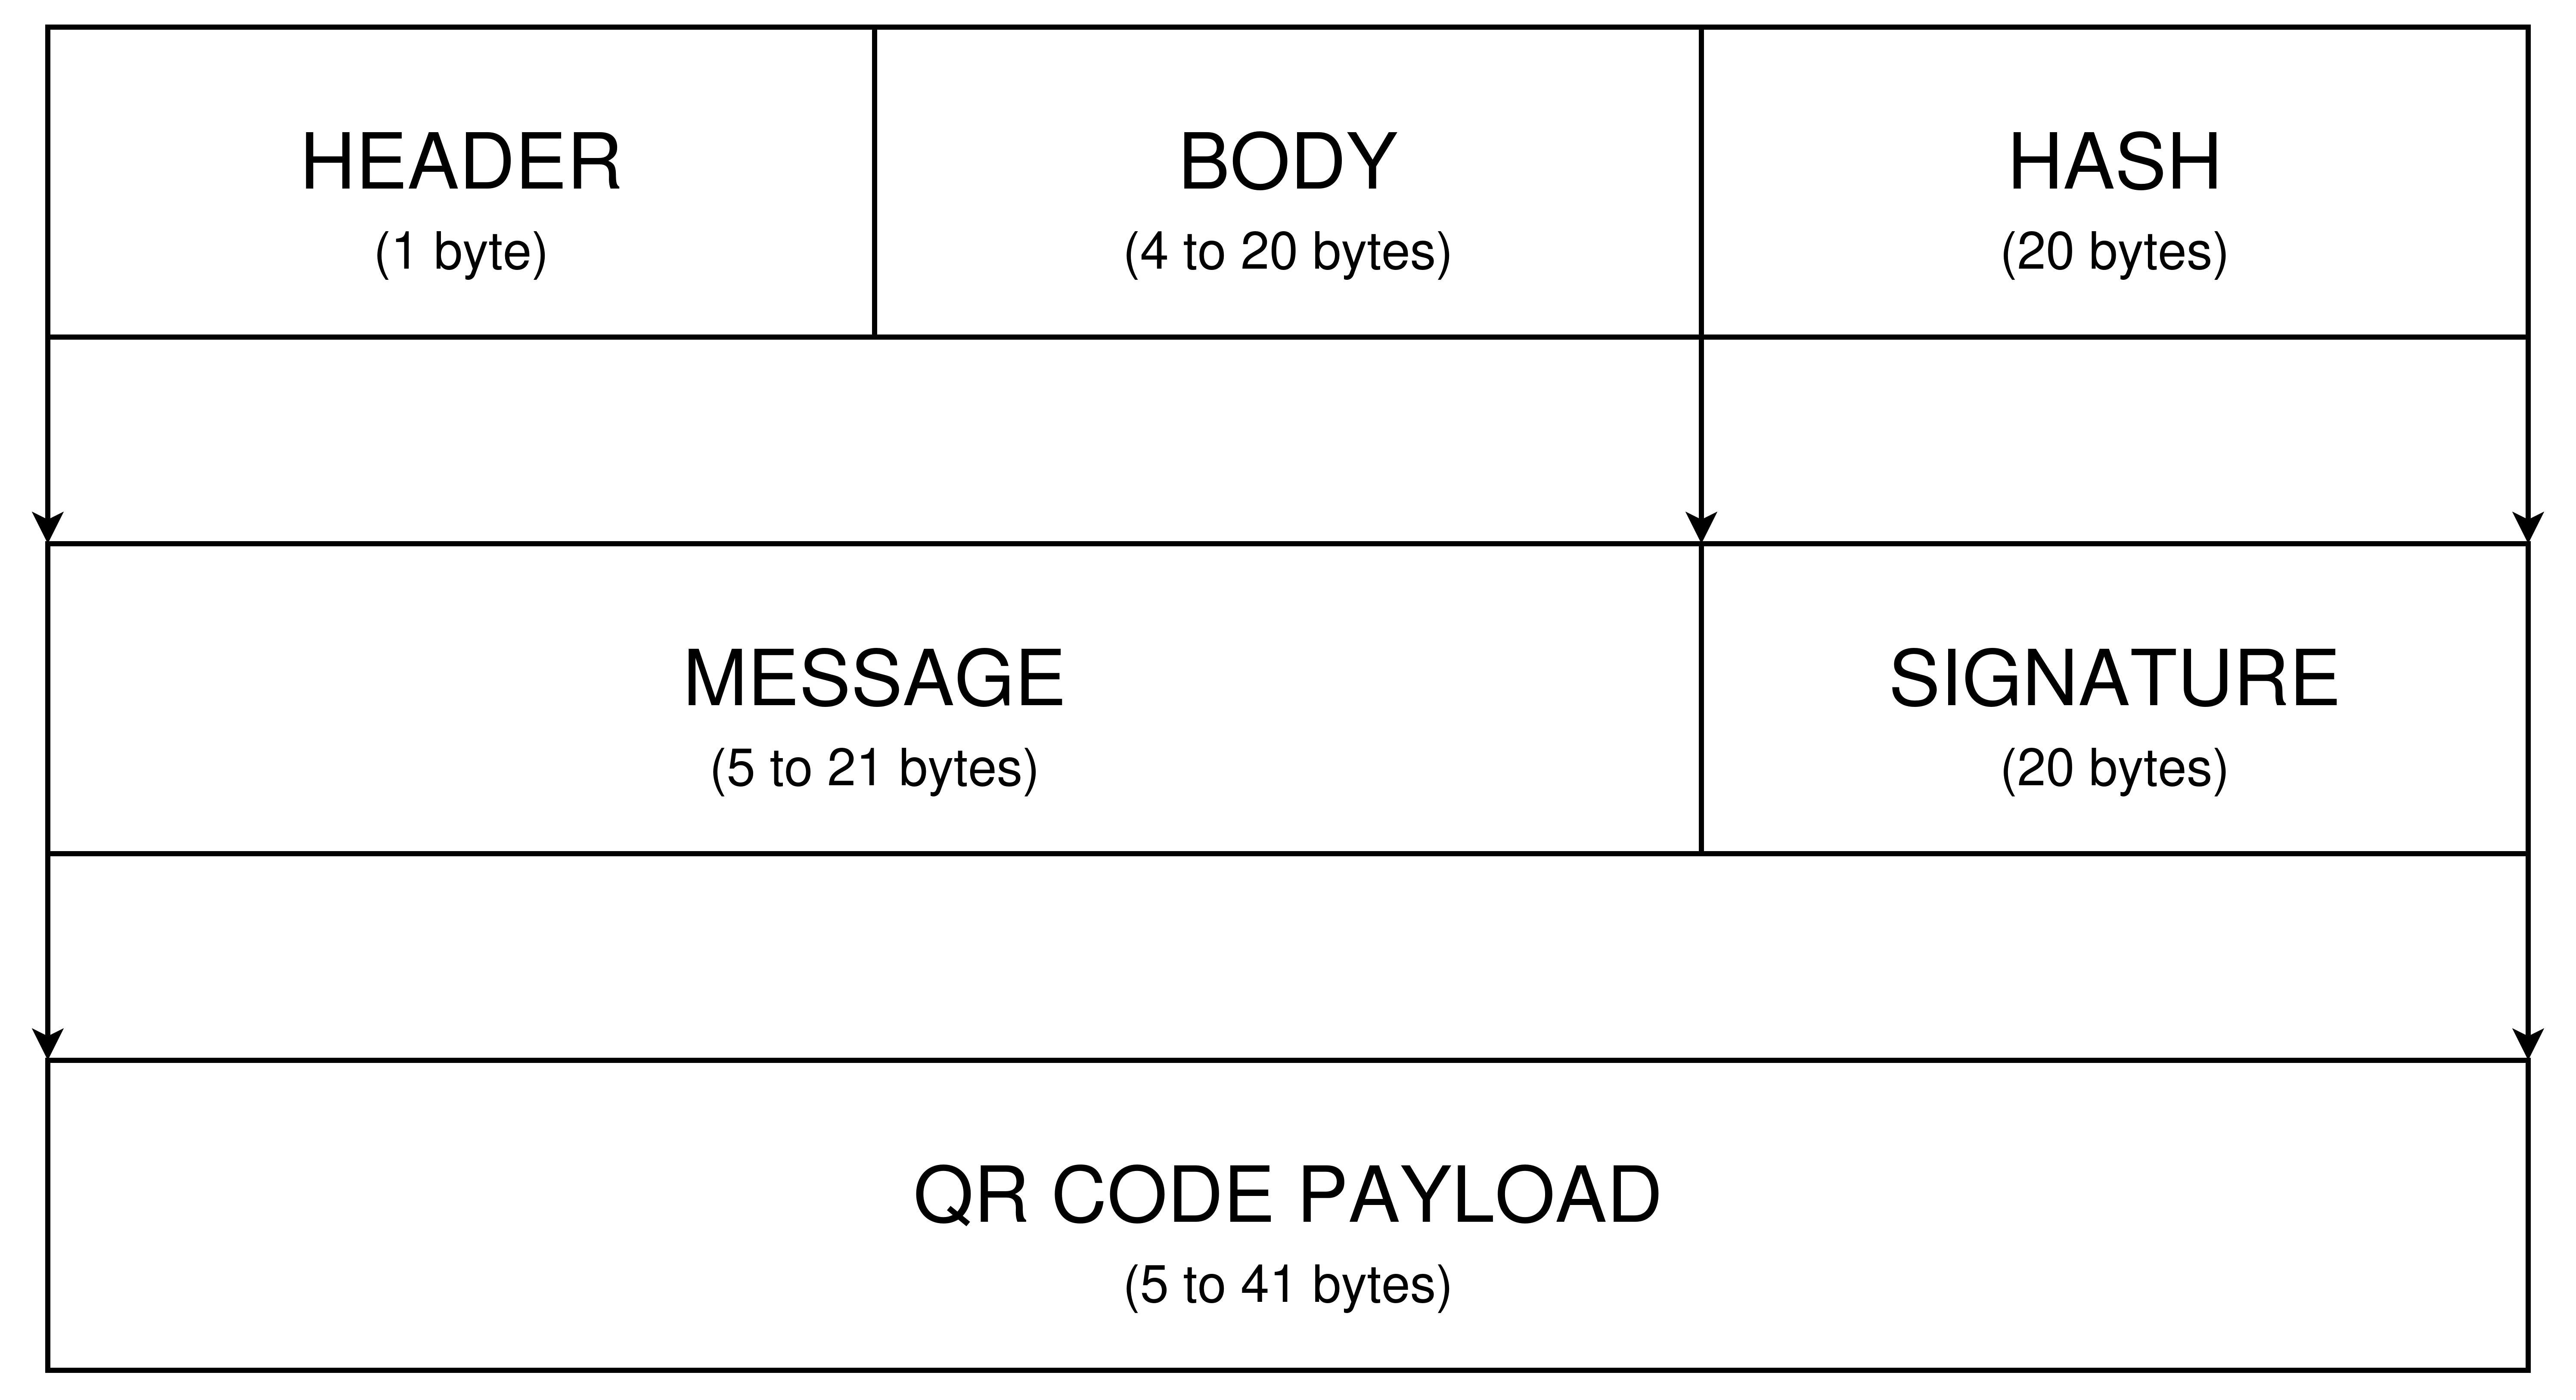
\includegraphics[width=10cm]{images/causp-lock-protocol-GENERAL_MESSAGE.png}
    \caption{Codificação do payload do QR Code}
    \label{fig:payload_encoding}
\end{figure}

Nesse contexto, denomina-se MESSAGE a concatenação de HEADER com BODY, nessa ordem (MESSAGE = HEADER + BODY), e SIGNATURE o HASH do payload. Dessa forma, a assinatura digital do QR Code considera como mensagem tanto o HEADER quanto o BODY (tipo de mensagem e dados da mensagem), o que permite verificar a integridade e autenticidade do QR Code, inviabilizando tentativas de adulteração ou falsificação de QR Codes existentes.

\subsection{MESSAGE TYPES}
Os QR Codes gerados pelo sistema web não são apenas os de acesso; há também QR Codes para sincronização de relógio do ESP32-CAM, configuração de novas chaves secretas e, por fim, QR Codes de debug, para testar o sistema sem alterar seu estado. Nosso protocolo estabelece 4 tipos de mensagem (MESSAGE\_TYPE):

\begin{enumerate}
    \item ACCESS (0): mensagens de acesso, que permitem ao cliente e administradores entrarem e saírem da sala.
    \item SYNC (1): mensagens de sincronização, para configurar o relógio interno do ESP32-CAM.
    \item CONFIG (2): mensagens de configuração, para configurar variáveis de ambiente e as chaves secretas HMAC-SHA1, para autenticação de mensagens.
    \item DEBUG (3): mensagens de depuração, para testar o dispositivo físico, sem alterar seu estado ou seus dados armazenados.
\end{enumerate}

Esses quatro tipos de mensagem recebem, cada um, um código MESSAGE\_TYPE padrão. ACCESS, SYNC, CONFIG e DEBUG recebem os códigos 0, 1, 2 e 3, respectivamente.

\subsection{OPERATION\_TYPES}
Enquanto o MESSAGE\_TYPE determina o tipo de mensagem, o OPERATION\_TYPE especifica mais a mensagem, ao explicitar que tipo de operação se deseja realizar. Por exemplo, os QR Codes de acesso são todos do tipo MESSAGE\_TYPE = 0 (ACCESS), mas há um QR Code para CHECK\_IN, que serve para abrir a fechadura e registar sua chegada, um CHECK\_OUT, para registrar saída da sala, e um BI\_ACCESS, que serve para entrar ou sair indistintamente. Em nosso protocolo, CHECK\_IN, CHECK\_OUT e BI\_ACCESS são denominadas ações. O tipo de uma ação (ACTION\_TYPE) é determinado pelo conjunto MESSAGE\_TYPE E OPERATION\_TYPE, conforme ilustram a tabela \ref{tab:operation_types_encoding} e a figura \ref{fig:header_encoding}.

\begin{table}
\centering
\vspace{0.5em}
\begin{tabular}{lll}
MESSAGE\_TYPE & OPERATION\_TYPE & ACTION\_TYPE \\ \hline
ACCESS & 0 & CHECK\_IN\\
ACCESS & 1 & CHECK\_OUT\\
ACCESS & 2 & BI\_ACCESS\\
SYNC & 0 & SET\_TIME\\
CONFIG & 0 & SET\_MASTER\_KEY\\
CONFIG & 1 & SET\_CONFIG\_KEY\\
CONFIG & 2 & SET\_ACCESS\_KEY\\
CONFIG & 3 & SET\_SYNC\_KEY\\
DEBUG & 0 & BLINK\_N\_TIMES\\
DEBUG & 1 & BLINK\_IF\_SYNC\\
\hline
\end{tabular}
\label{tab:operation_types_encoding}
\caption{Codificação do OPERATION\_TYPE}
\end{table}

Essa configuração permite adicionar facilmente novas ações conforme a necessidade, sem prejudicar a lógica e a numeração das já existentes. por exemplo, se desejarmos adicionar um quarto tipo de acesso, basta criar uma ação com MESSAGE\_TYPE = ACCESS e OPERATION\_TYPE = 3, o que não modifica a codificação das demais ações já cadastradas. Além disso, essa divisão facilita o entendimento do sistema, ao agrupar semanticamente as ações por grupo e depois especificá-las melhor com o campo OPERATION\_TYPE.

\subsection{HEADER}
A seção HEADER é o cabeçalho da mensagem, que identifica seu tipo e que operação se deseja fazer. Ela contém dois campos: (i) MESSAGE\_TYPE e (ii) OPERATION\_TYPE. Cada campo é codificado com 4 bits, de forma que o HEADER tenha exatamente 1 byte (8 bits) de tamanho. O MESSAGE\_TYPE ocupa os 4 bits mais significativos do byte de HEADER, enquanto que OPERATION\_TYPE ocupa os 4 bits menos significativos. Por exemplo, a ação SET\_CONFIG\_KEY possui MESSAGE\_TYPE = 2 = 0010 (binário) e OPERATION\_TYPE = 1 = 0001 (binário), portanto, o HEADER correspondente é 0010 0001 (binário) = 21 (hexadecimal), conforme ilustra a tabela \ref{tab:header_encoding}

\begin{figure}
    \centering
    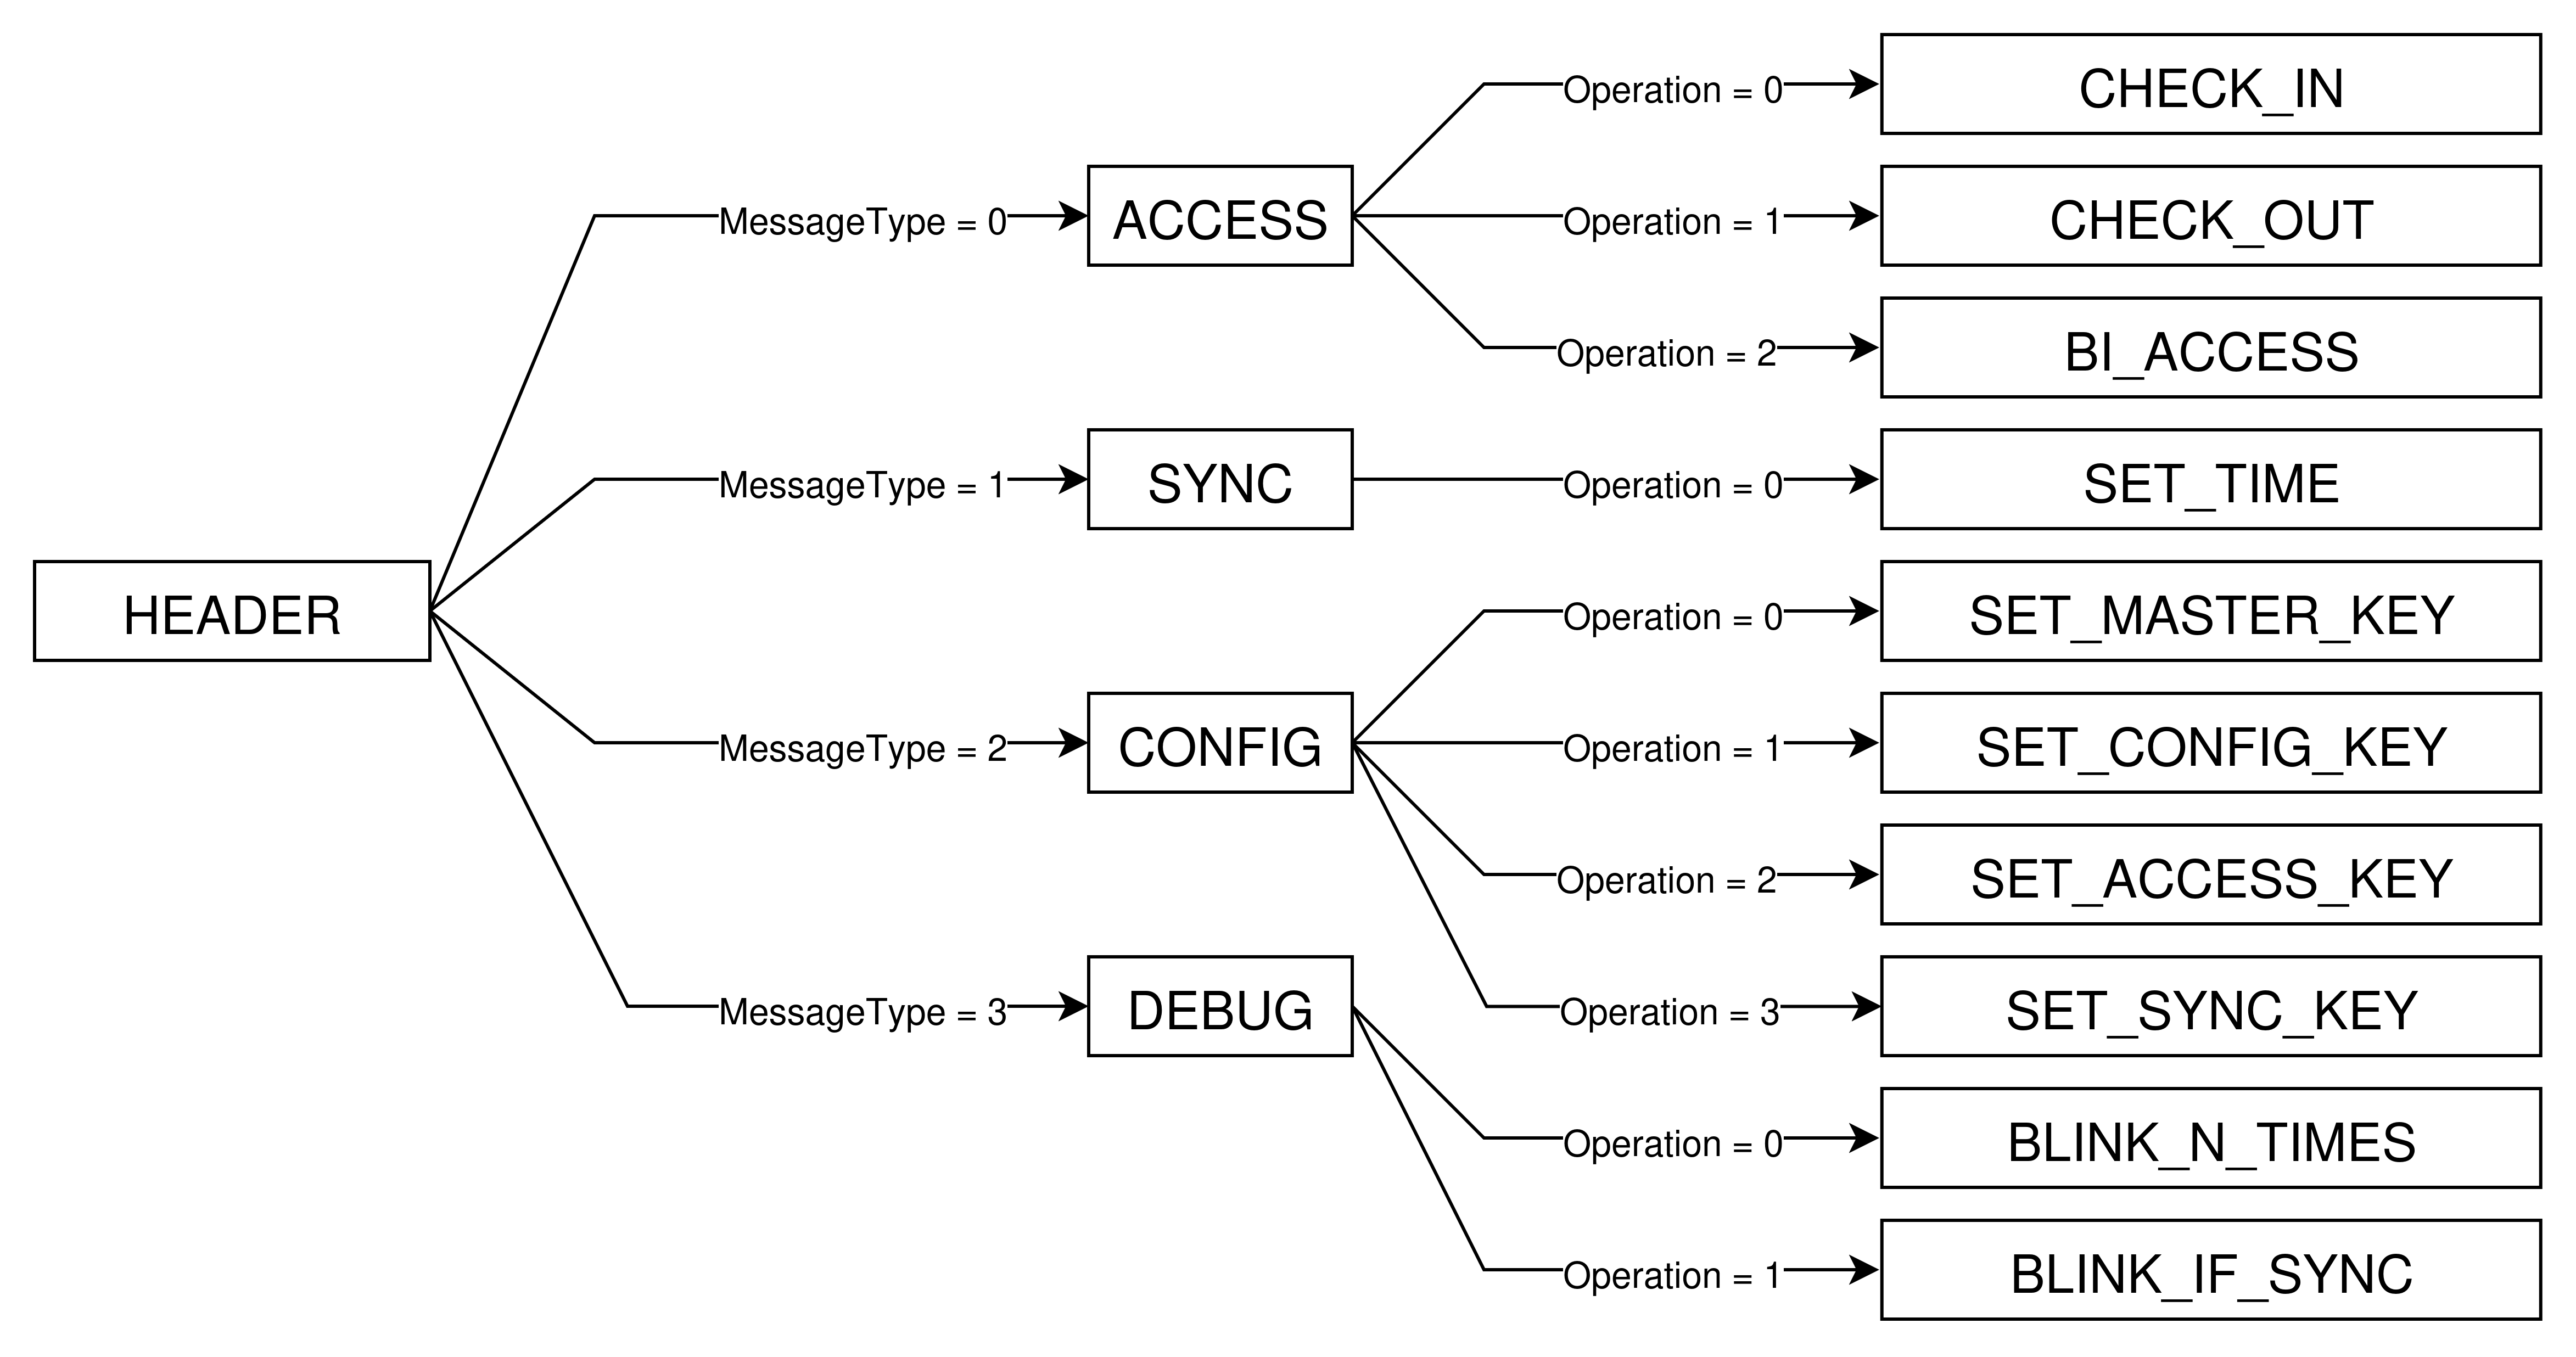
\includegraphics[width=14cm]{images/causp-lock-protocol-HEADER_ENCODING.png}
    \caption{Codificação do HEADER}
    \label{fig:header_encoding}
\end{figure}

% Please add the following required packages to your document preamble:
% \usepackage{booktabs}
\begin{table}
\centering
\begin{tabular}{@{}lllllll@{}}
\multicolumn{3}{l}{MESSAGE\_TYPE} & \multicolumn{2}{l}{OPERATION\_TYPE} & \multicolumn{2}{l}{HEADER} \\ \midrule
name        & hex      & bin      & hex              & bin              & hex       & bin            \\ \midrule
ACCESS      & 0        & 0000     & 0                & 0000             & 00        & 0000 0000      \\
ACCESS      & 0        & 0000     & 1                & 0001             & 01        & 0000 0001      \\
ACCESS      & 0        & 0000     & 2                & 0010             & 02        & 0000 0010      \\
SYNC        & 1        & 0001     & 0                & 0000             & 10        & 0001 0000      \\
CONFIG      & 2        & 0010     & 0                & 0000             & 20        & 0010 0000      \\
CONFIG      & 2        & 0010     & 1                & 0001             & 21        & 0010 0001      \\
CONFIG      & 2        & 0010     & 2                & 0010             & 22        & 0010 0010      \\
CONFIG      & 2        & 0010     & 3                & 0011             & 23        & 0010 0011      \\
DEBUG       & 3        & 0011     & 0                & 0000             & 30        & 0011 0000      \\
DEBUG       & 3        & 0011     & 1                & 0001             & 31        & 0011 0001      \\ \bottomrule
\end{tabular}
\caption{Codificação do HEADER}
\label{tab:header_encoding}
\end{table}

\subsection{BODY}
O BODY é uma seção, de tamanho variável, que contém os dados de cada mensagem. Que campos são encontrados nela e sua interpretação dependem do MESSAGE\_TYPE. Por exemplo, em QR Codes de acesso, o BODY deve conter o id do usuário (user\_id) e o instante de tempo em que se gerou o código (generated\_at); em QR Codes de sincronização, o BODY deve ter apenas o novo tempo, que se deseja configurar no ESP32-CAM. Os dados do BODY para cada tipo de QR Code estão descritos na tabela \ref{tab:body_encoding}.

% Please add the following required packages to your document preamble:
% \usepackage{booktabs}
\begin{table}
\centering
\begin{tabular}{@{}ccccc|c@{}}
\toprule
\begin{tabular}[c]{@{}c@{}}BODY\\ {[}0:3{]}\end{tabular}     & \begin{tabular}[c]{@{}c@{}}BODY\\ {[}4:7{]}\end{tabular}     & \begin{tabular}[c]{@{}c@{}}BODY\\ {[}8:11{]}\end{tabular}     & \begin{tabular}[c]{@{}c@{}}BODY\\ {[}12:15{]}\end{tabular}     & \begin{tabular}[c]{@{}c@{}}BODY\\ {[}16:19{]}\end{tabular}     & MESSAGE\_TYPE \\ \midrule
user\_id                                                     & generated\_at                                                & -                                                             & -                                                              & -                                                              & ACCESS        \\
sync\_time                                                   & -                                                            & -                                                             & -                                                              & -                                                              & SYNC          \\
\begin{tabular}[c]{@{}c@{}}new\_key\\ {[}0:3{]}\end{tabular} & \begin{tabular}[c]{@{}c@{}}new\_key\\ {[}4:7{]}\end{tabular} & \begin{tabular}[c]{@{}c@{}}new\_key\\ {[}8:11{]}\end{tabular} & \begin{tabular}[c]{@{}c@{}}new\_key\\ {[}12:15{]}\end{tabular} & \begin{tabular}[c]{@{}c@{}}new\_key\\ {[}16:19{]}\end{tabular} & CONFIG        \\
blink\_num                                                   & -                                                            & -                                                             & -                                                              & -                                                              & DEBUG         \\
sync\_time                                                   & -                                                            & -                                                             & -                                                              & -                                                              & DEBUG         \\ \bottomrule
\end{tabular}
\caption{Codificação do BODY por MESSAGE\_TYPE}
\label{tab:body_encoding}
\end{table}

Na notação da tabela, X[a:b] indica os bytes índice a, a + 1, a + 2, ..., b - 3, b - 2, b - 1 de X. Portanto, BODY[0:3] são os quatro primeiros bytes do BODY; BODY[4:7], os 4 bytes seguintes, e assim por diante. Em nossa implementação, consideramos as chaves com exatos 20 bytes; mas, a princípio, esse número é arbitrário, já que o HMAC-SHA1 aceita chaves de tamanho arbitrário.Deve-se notar que há 5 campos distintos:

\begin{enumerate}
    \item user\_id (4 bytes): o identificador único do usuário, como um inteiro de 32 bits.
    \item generated\_at (4 bytes): o instante de tempo em que o código foi gerado, como tempo POSIX em 32 bits.
    \item new\_key: a nova chave HMAC-SHA1 que sobrescreverá a antiga, registrada no ESP32-CAM.
    \item blink\_num: número de vezes em que o ESP32-CAM deve piscar, caso se apresente esse QR Code.
    \item sync\_time: o instante de tempo para o qual será setado o relógio interno do ESP32-CAM no SYNC ou para teste de sincronismo no DEBUG, como tempo POSIX em 32 bits.
\end{enumerate}

Um aspecto importante é que o tempo é codificado em um POSIX de apenas 4 bytes (32 bits). Isso limita a solução, pois ela só pode representar instantes de tempo aproximadamente até janeiro 2038. No entanto, para o projeto, optou-se por manter esse tempo dessa maneira mesmo assim, pois isso permitiu manter os códigos de acesso no QR Code versão 2, que é consideravelmente menor que o da versão 3; isso é essencial pois QR Codes mais simples são mais fáceis de serem lidos pela câmera OV2640.

\subsection{HASH}
O HASH é a seção do payload que contém a assinatura digital HMAC-SHA1, com exatos 20 bytes. Ela está presente em todos os MESSAGE\_TYPE, exceto para os de DEBUG, por não exigirem autenticação. Ela é colocada sempre ao final do payload.

\section{Sistema Físico}
O diagrama elétrico está descrito na figura \ref{fig:eletrical_diagram}. O sistema fisicamente possui um ESP32-CAM, alimentado por uma fonte de 5V e 1A (máx.), ligada na rede elétrica, e conectado a uma câmera OV2640. Um pino GPIO do ESP32-CAM denominado aqui de UNLOCK é responsável por destravar a fechadura elétrica; quando em HIGH, a interpretação do sinal é a de destravar e, quando em LOW, o contrário.

No entanto, não é possível acionar a fechadura diretamente com o sinal do microcontrolador, porque, enquanto a fechadura demanda 12V e 1A por 1s, ele fornece apenas 3.3V e menos de 1A. Para contornar esse problema, emprega-se um relé eletromecânico, que interrompe condicionalmente um fio, conectado à fechadura elétrica e a uma fonte chaveada de 12V e 5A.

Mas, mesmo assim, o sinal do ESP32-CAM não é suficiente sequer para acionar o relé; por isso, empregou-se o transistor 2N2222 num circuito amplificador de sinal, utilizando a própria fonte chaveada de 12V como VCC; o sinal de 3.3V então é amplificado para cerca de 11V, que já é capaz de acionar o relé.

\begin{figure}[H]
    \centering
    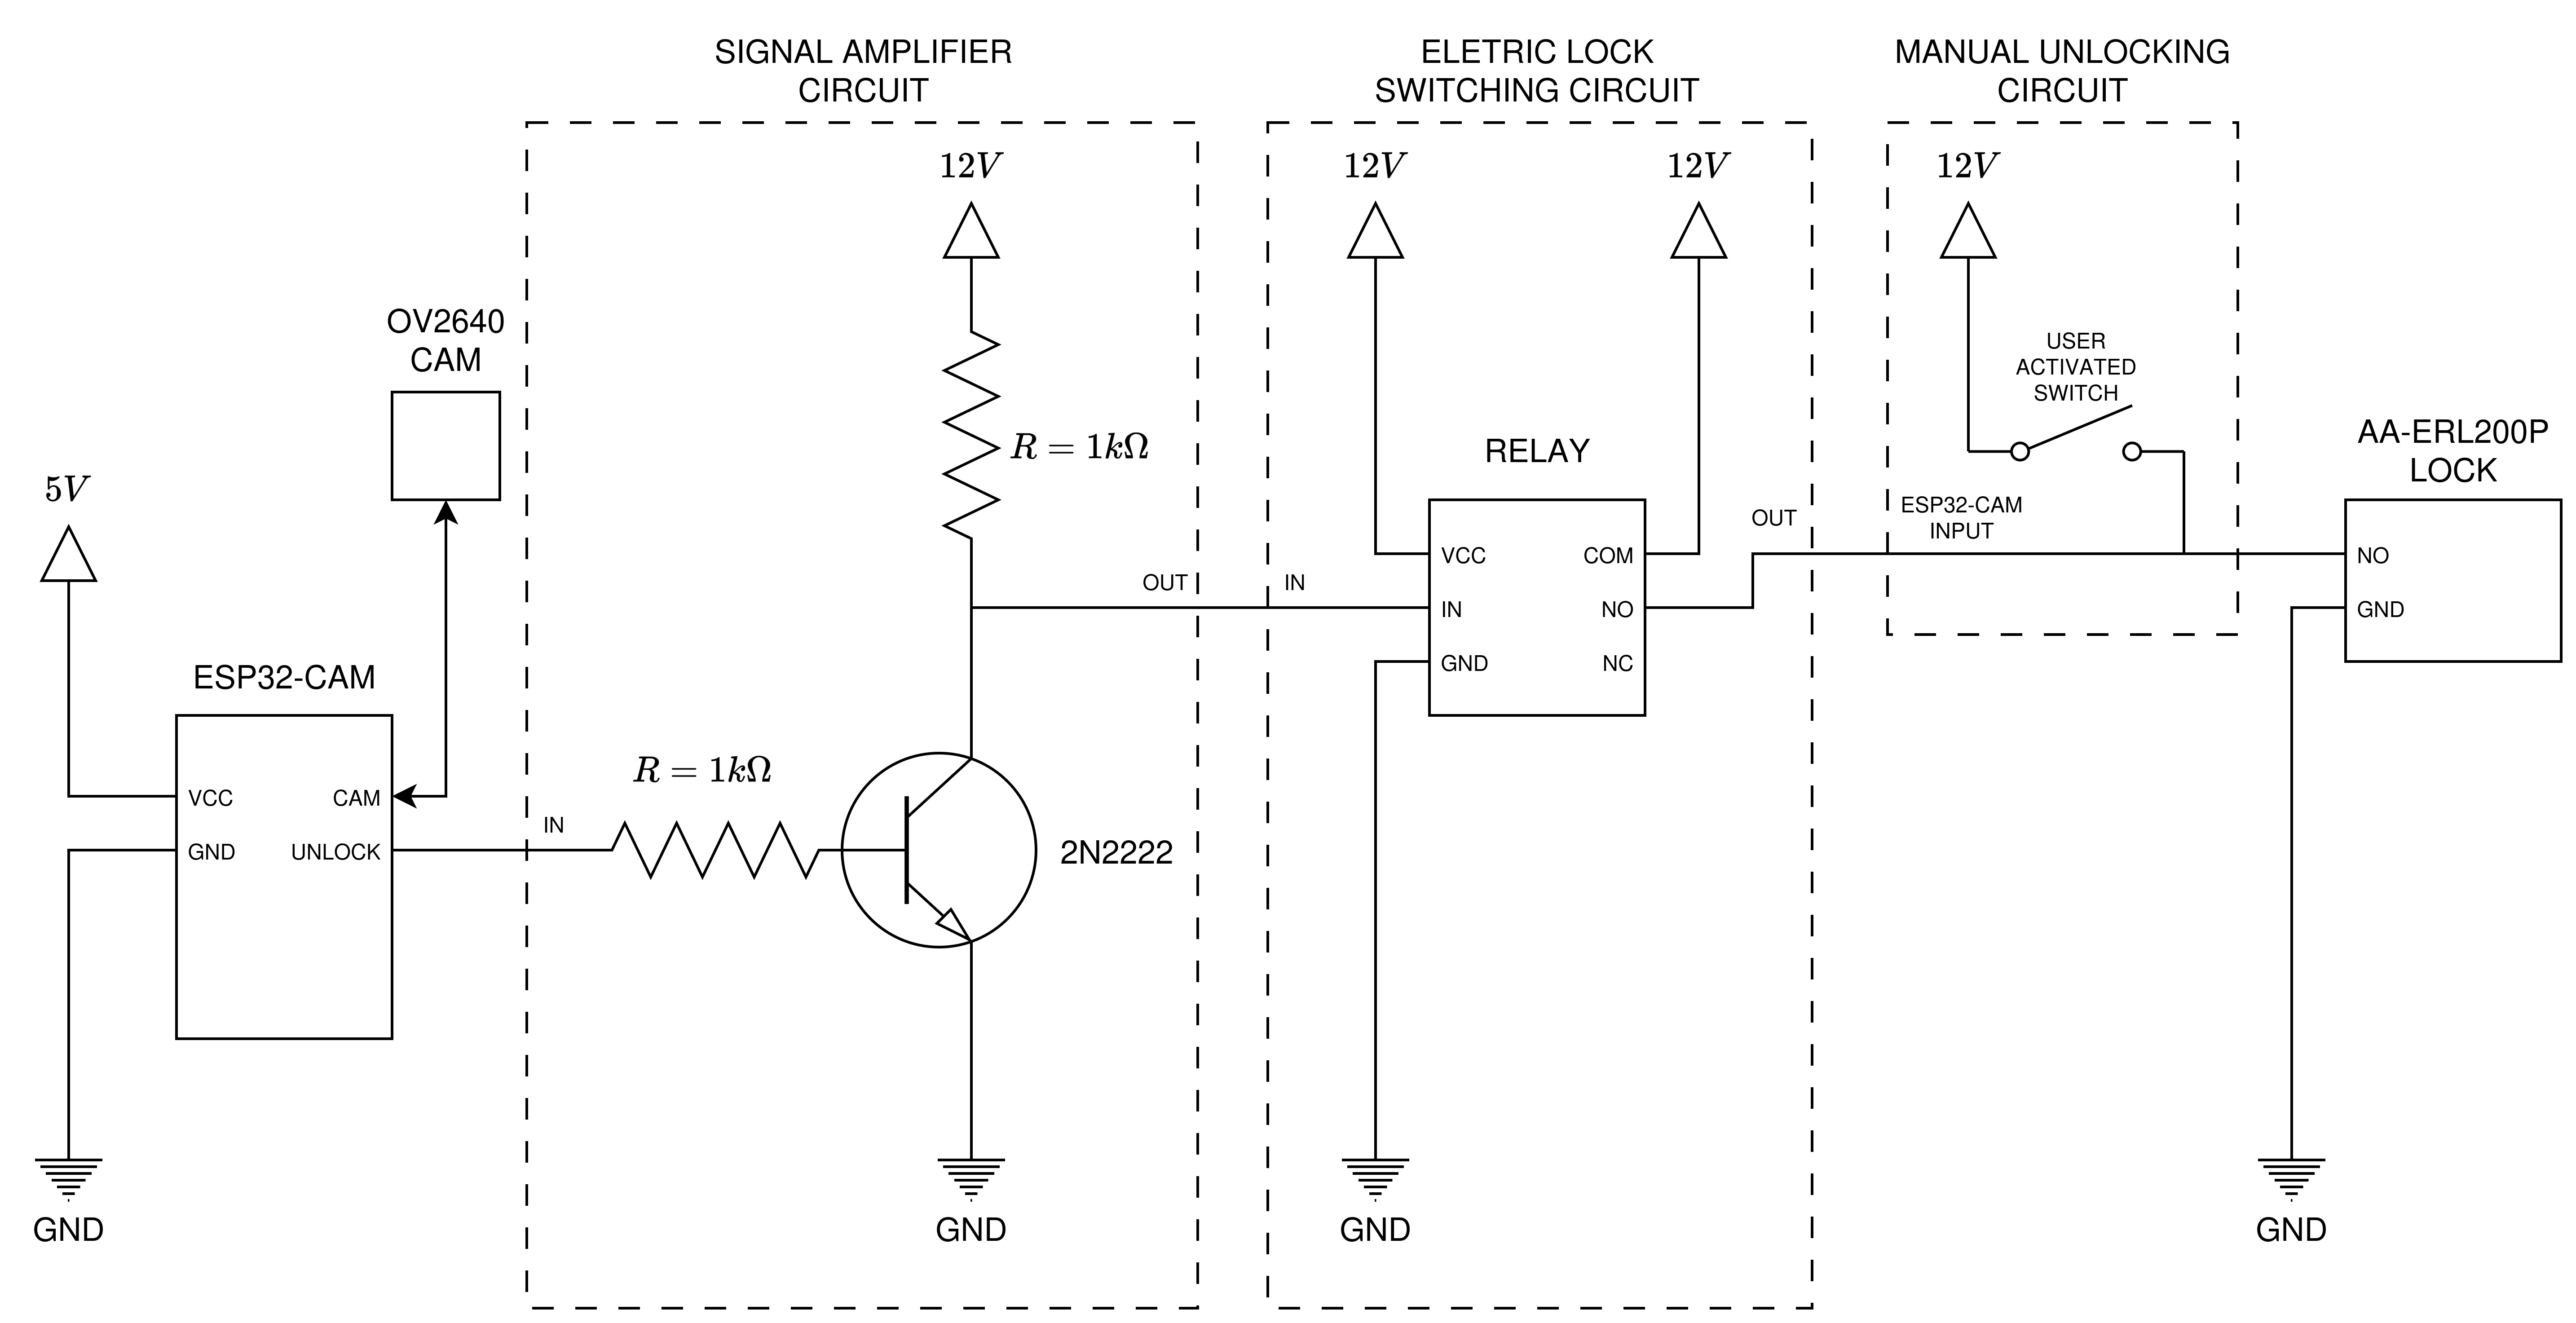
\includegraphics[width=14cm]{images/causp-lock-protocol-ELETRIC_DIAGRAM.png}
    \caption{Diagrama elétrico}
    \label{fig:eletrical_diagram}
\end{figure}

Note na figura \ref{fig:eletrical_diagram} um sistema de switch, na proximidade da fechadura elétrica. Esse switch possui a função de permitir saída da sala independentemente do ESP32-CAM, por exemplo, em caso de falha dele ou erro lógico. Isso impede que o usuário fique preso na sala, após adentrá-la, sendo, portanto, um mecanismo de segurança.

\section{Protótipo}
Implementou-se o sistema CAUSP-LOCK projetado num protótipo simples, como prova de conceito do projeto. A montagem física está explicitada na figura \ref{fig:protótipo}, que implementa o diagrama elétrico da figura \ref{fig:eletrical_diagram}, apenas com a diferença de não ter o switch de acionamento interno, por simplicidade.

\begin{figure}[H]
    \centering
    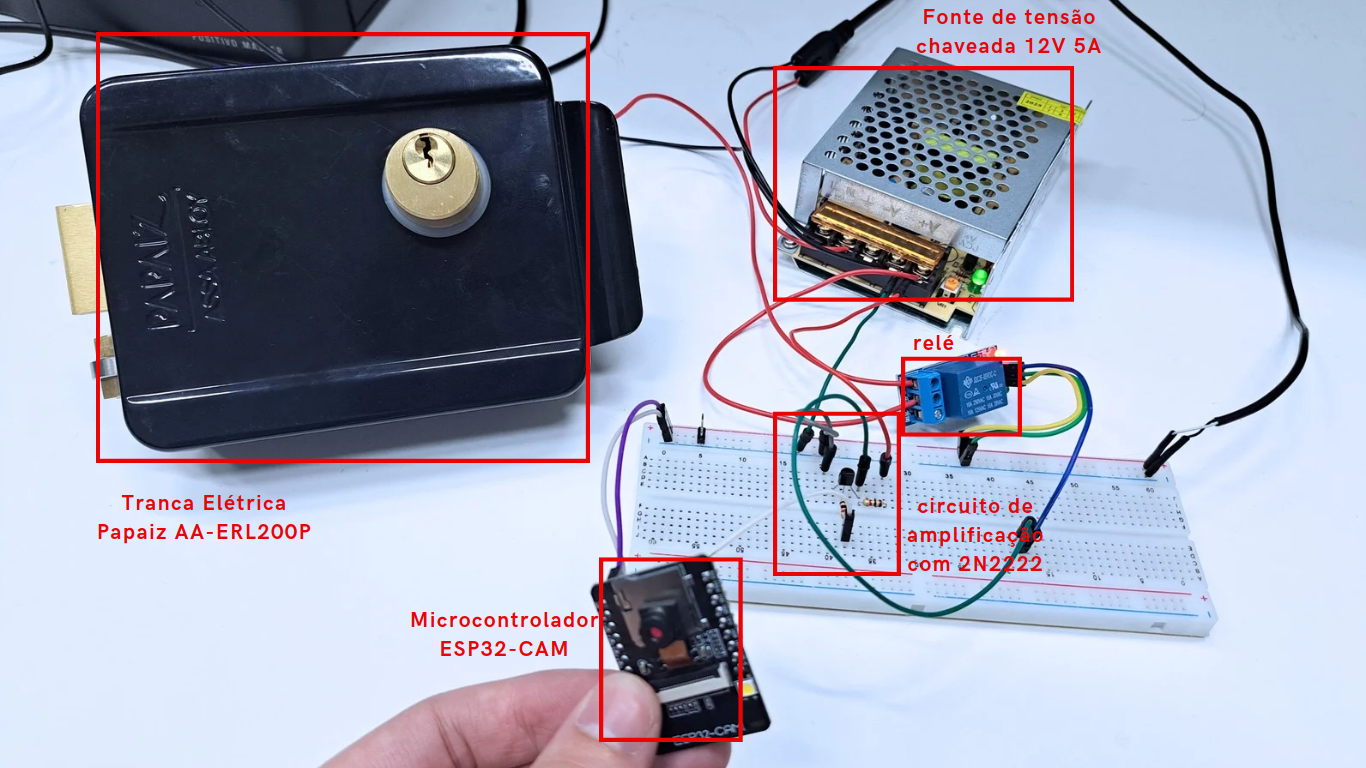
\includegraphics[width=12cm]{images/protótipo_anotado.png}
    \caption{Protótipo como prova de conceito}
    \label{fig:protótipo}
\end{figure}

Testou-se o protótipo para um caso simples, de validar um QR Code de acesso, sem se preocupar com sua expiração mas necessariamente decodificando todas suas informações, e, finalmente, acionando a fechadura elétrica, abrindo-a para o usuário. O teste foi um sucesso e pode ser visto no vídeo abaixo:

\href{https://youtu.be/gl5iByZ4_28}{https://youtu.be/gl5iByZ4\_28}

\section{ESP32-CAM}
Esta sessão destina-se a explicar as especificidades técnicas do ESP32-CAM, que o tornam ideal para o projeto. O módulo ESP32‑CAM é baseado no chip \textbf{ESP32‑S}, que utiliza o microcontrolador \textbf{ESP32} da Espressif Systems. O componente central é o microprocessador \textbf{Tensilica Xtensa LX6}, de 32 bits, configurável para \textbf{dual‑core} (inicialmente em até dois núcleos) ou \textbf{single‑core} na variante ESP32‑S0WD 

\subsection{Arquitetura, desempenho e recursos do processador}
O ESP32-CAM utiliza o processador Xtensa LX6, que geralmente opera com dois núcleos, permitindo concorrência eficiente entre tarefas paralelas como captura de imagem, compressão JPEG e transmissão Wi-Fi. A frequência de operação é ajustável entre 80 MHz e 240 MHz, sendo este último o valor máximo recomendado. Nessa configuração, o processador alcança aproximadamente 994 pontos no benchmark CoreMark em dual-core, o que corresponde a cerca de $\approx$ 4{,}14 CoreMark/MHz. Sua performance teórica atinge até 600 DMIPS, e há ainda um coprocessador ULP (Ultra Low Power) integrado, capaz de realizar operações como leitura de ADCs ou comparações durante o modo de deep-sleep, sem a necessidade de ativar os núcleos principais.

O microcontrolador conta com 520 KiB de SRAM para execução de código e dados em tempo real, além de aproximadamente 448 KiB de ROM utilizada para armazenar o firmware de boot e rotinas do sistema. Há também cerca de 16 KiB de memória RTC SRAM acessível durante os modos de sono profundo, permitindo que o coprocessador ULP opere mesmo com o sistema principal desligado.

O ESP32 oferece suporte nativo ao sistema operacional FreeRTOS, permitindo execução preemptiva de tarefas com gerenciamento de threads em ambos os núcleos. Esse recurso possibilita a divisão eficiente de tarefas, como manter a comunicação via Wi-Fi em um núcleo enquanto o outro processa sinais da câmera. Adicionalmente, o chip suporta DVFS (Dynamic Voltage and Frequency Scaling), ajustando dinamicamente a frequência e a tensão de operação de acordo com a carga do sistema, o que contribui para o balanceamento entre desempenho e economia de energia.

Em termos de segurança e aceleração de tarefas criptográficas, o processador conta com boot seguro e criptografia de memória flash. Também estão integrados aceleradores de hardware para algoritmos como AES, SHA-2, RSA e curvas elípticas (ECC), além de um gerador de números aleatórios (RNG), o que garante robustez em aplicações seguras conectadas à internet.


\begin{table}[H]
    \centering
    % Adicionamos o comando abaixo para aumentar o espaçamento das linhas
    \renewcommand{\arraystretch}{1.5}
    \label{tab:esp32_specs_spaced}
    \begin{tabular}{c >{\centering\arraybackslash}p{10cm}}
        \toprule
        \textit{\textbf{Item}} & \textit{\textbf{Especificação}} \\
        \midrule
        \textbf{CPU} & Tensilica Xtensa LX6, 32 bit, arquitetura Harvard \\
        \textbf{Núcleos} & Dual-core (até 240 MHz) ou single-core (ESP32‑S0WD) \\
        \textbf{Desempenho} & 994 CoreMark dual-core; $\approx$ 600 DMIPS \\
        \textbf{Memória interna} & 520 KiB SRAM; 448 KiB ROM; 16 KiB RTC SRAM \\
        \textbf{Coprocessador ULP} & Suporte a ADC e comparações durante deep-sleep \\
        \textbf{Criptografia} & AES, SHA-2, RSA, ECC; RNG embutido \\
        \textbf{Modo de clock} & 80–240 MHz com DVFS \\
        \textbf{Sistema operacional} & FreeRTOS com multitarefa \\
        \bottomrule
    \end{tabular}
    \caption{Especificações principais do processador Xtensa LX6 (ESP32)}
\end{table}


\subsection{Pipeline de 7 Estágios do Xtensa LX6}

O processador 	\textbf{Xtensa LX6}, utilizado no ESP32, possui um pipeline de 7 estágios que permite alta frequência de operação com instruções de baixa latência. A seguir, apresenta-se um diagrama simplificado dos estágios:

\begin{figure}
\centering
% --- Início das Modificações ---
\begin{tikzpicture}[
    node distance=0.5cm, % Reduz a distância base entre os nós
    every node/.style={
        draw,
        minimum height=1cm,
        text width=2.2cm, % Define uma largura máxima para o texto
        align=center      % Alinha o texto quebrado ao centro
    }
]
% --- Fim das Modificações ---

% Usando a sintaxe moderna 'right=of <node>' para melhor posicionamento
\node (IF) {IF - Instruction Fetch};
\node (ID) [right=of IF] {ID - Instruction Decode};
\node (OF) [right=of ID] {OF - Operand Fetch};
\node (EX) [right=of OF] {EX - Execute};
\node (MA) [right=of EX] {MA - Memory Access};
\node (WB) [right=of MA] {WB - Write Back};

% Posicionando o nó CT abaixo de EX
\node (CT) [below=of EX, yshift=-0.5cm] {CT - Commit Trap};

% As setas permanecem as mesmas
\draw[->] (IF) -- (ID);
\draw[->] (ID) -- (OF);
\draw[->] (OF) -- (EX);
\draw[->] (EX) -- (MA);
\draw[->] (MA) -- (WB);
\draw[->, dashed] (EX.south) -- (CT.north); % Conexão mais precisa

\end{tikzpicture}
\caption{Pipeline simplificado de 7 estágios do Xtensa LX6.}
\end{figure}


O pipeline é composto pelos estágios: \textbf{IF} (Instruction Fetch), que busca a próxima instrução da memória; \textbf{ID} (Instruction Decode), que decodifica a instrução; \textbf{OF} (Operand Fetch), que busca operandos dos registradores; \textbf{EX} (Execute), que realiza a operação aritmética ou lógica; \textbf{MA} (Memory Access), que acessa a memória caso necessário; \textbf{WB} (Write Back), que escreve o resultado de volta no registrador; e \textbf{CT} (Commit Trap), que verifica e lida com interrupções e exceções.

\subsection{Exemplo em Assembly Xtensa (manipulação de pilha)}

\begin{lstlisting}[
    language={[x86masm]Assembler},
    caption={Função simples em Xtensa Assembly com manipulação de pilha},
    xleftmargin=\fill, % Adicionado para centralizar
    xrightmargin=\fill  % Adicionado para centralizar
]
entry    a1, 32         ; aloca 32 bytes na pilha, atualiza SP
movi     a2, 10         ; move valor 10 para a2
s32i     a2, a1, 0      ; salva a2 no topo da pilha (offset 0)
call0    func           ; chamada de funcao sem salvar janelas

func:
l32i     a3, a1, 0      ; carrega valor da pilha para a3
add      a3, a3, a3     ; duplica o valor
ret
\end{lstlisting}

\textbf{Explicação}

A execução do código se baseia em três instruções principais. A instrução \texttt{entry} é responsável por reservar o espaço necessário para variáveis locais na pilha. Em seguida, \texttt{call0} é utilizada para realizar chamadas de função de forma otimizada, sem salvar a janela de registradores. Por fim, as instruções \texttt{s32i} e \texttt{l32i} manipulam os dados diretamente, salvando e carregando valores da pilha.

\subsection{Comparativo com ARM Cortex-M e RISC-V RV32IMC}

\begin{table}[H]
    \centering
    % 1. Aumenta o espaçamento vertical entre as linhas
    \renewcommand{\arraystretch}{1.5}
    
    
    \label{tab:comparativo_arqs}
    
    % 2. Usa 'tabularx' para a tabela caber na página e 'X' para colunas com quebra de linha
    \begin{tabularx}{\textwidth}{l X X X}
        \toprule
        \textbf{Característica} & \textbf{Xtensa LX6 (ESP32)} & \textbf{ARM Cortex-M4} & \textbf{RISC-V RV32IMC} \\
        \midrule
        ISA                       & Xtensa (proprietária)       & ARMv7E-M                & RV32IMC (open-source) \\
        Arquitetura               & Harvard, dual-core          & Harvard, single-core    & Von Neumann/Harvard opcional \\
        Pipeline                  & 7 estágios                  & 3 a 6 estágios          & 5 estágios (tip.) \\
        Clock máximo              & 240 MHz                     & 120 MHz                 & 100--150 MHz \\
        FPU                       & Opcional                    & Presente (M4F)          & Opcional \\
        Consumo                   & Moderado (com modos sleep)  & Baixo                   & Muito baixo \\
        Debug                     & JTAG, OpenOCD               & SWD, DWT, ITM           & JTAG, OpenOCD \\
        Suporte RTOS              & FreeRTOS nativo             & CMSIS + FreeRTOS        & FreeRTOS, Zephyr \\
        Licenciamento             & Licença Espressif/Tensilica & ARM (licenciado)        & Open-source \\
        \bottomrule
    \end{tabularx}
    \caption{Comparativo entre as arquiteturas Xtensa, ARM e RISC-V}
\end{table}

O Xtensa LX6 se destaca por seu alto desempenho e flexibilidade, sendo adequado para aplicações embarcadas com requisitos de conectividade, processamento de imagem e resposta em tempo real, como é o caso do ESP32-CAM. Em termos didáticos, permite explorar multitarefa em dual-core, modos de economia de energia, co-processadores, extensões ISA e manipulação de pilha sem instruções dedicadas.

\end{document}